\section{Evaluation}
\subsection{Testbench}
To test the pixel circuit we use a testbench that applies parameterized biases, which are settable through the ADE
environment for quick bias tuning. The ON and OFF outputs of the pixel to the CA and
RA inputs, such that the pixel resets itself when an event is generated. The testbench also contains separated power
supplies for the analog and digital parts of the pixel, as well as the testbench itself. 
The bias generators are shown in Fig.~\ref{fig:tb-bias} and the connections for the pixel are shown in Fig.~\ref{fig:tb-pixel}.

We generated the input waveforms for the circuit using a piecewise linear current source for the input photocurrent
and a piecewise linear voltage source for the global reset. We evaluate the pixel on a change in contrast of a 
factor 3.3, from 10 pA to 33 pA. The 10 pA input current is held for the first 5 ms of the simulation while the pixel is reset,
then it is ramped up to 33 pA in 5 ms to simulate an operating frequency of 100 Hz. After the ramp up, the 
input current stays constant for 5 ms while the pixel is reset again, before it ramps back down to 10 pA.

The input signals as well as the pixel output response of 12 ON and 12 OFF events is shown in Fig.~\ref{fig:pixel-response}. 
\begin{figure}
    \center
    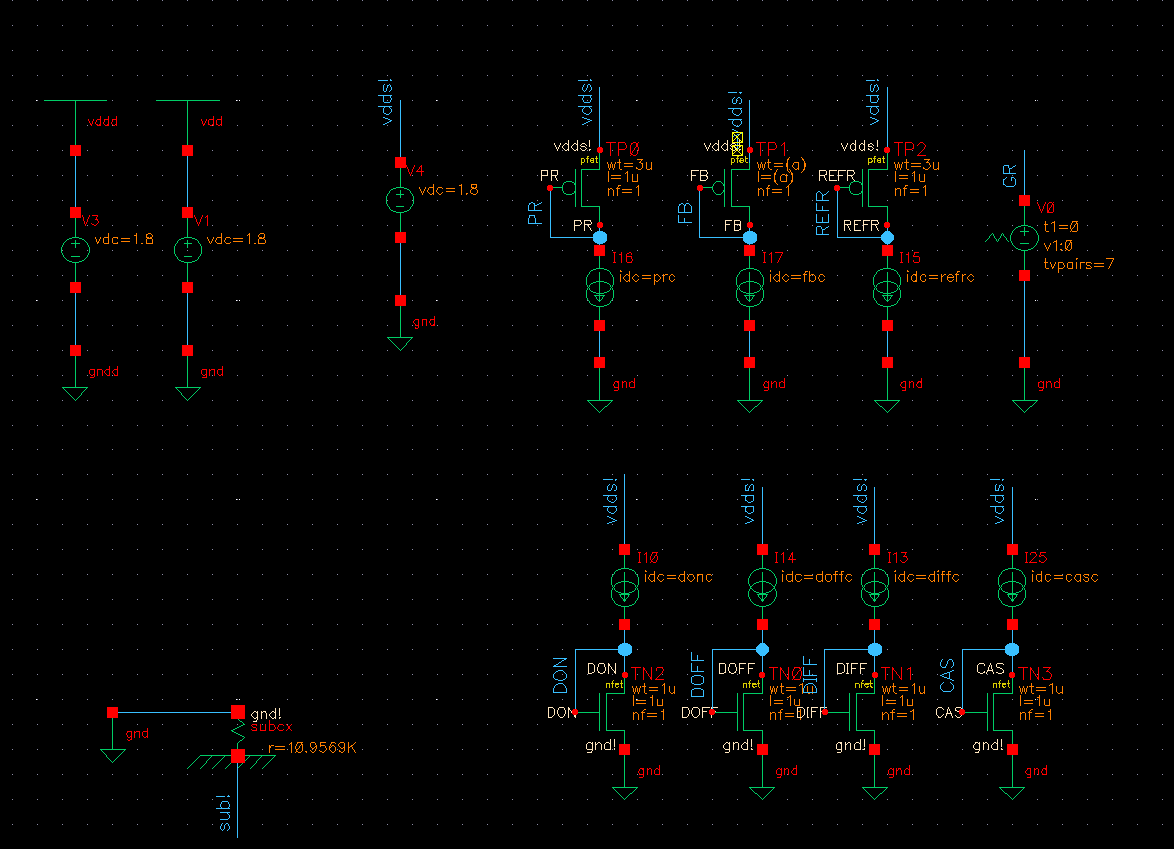
\includegraphics[width=\textwidth]{pixel_tb_bias.png}
    \caption{Pixel testbench bias generators and power supplies. \texttt{vdd} supplies the analog parts of the pixel
    subcircuit, \texttt{vddd} supplies the digital part of the pixel and \texttt{vdds} supplies the testbench. The
    supplies for the testbench and pixel are separated to facilitate accurate power consumption measurement.}
    \label{fig:tb-bias}
\end{figure}
\begin{figure}
    \center
    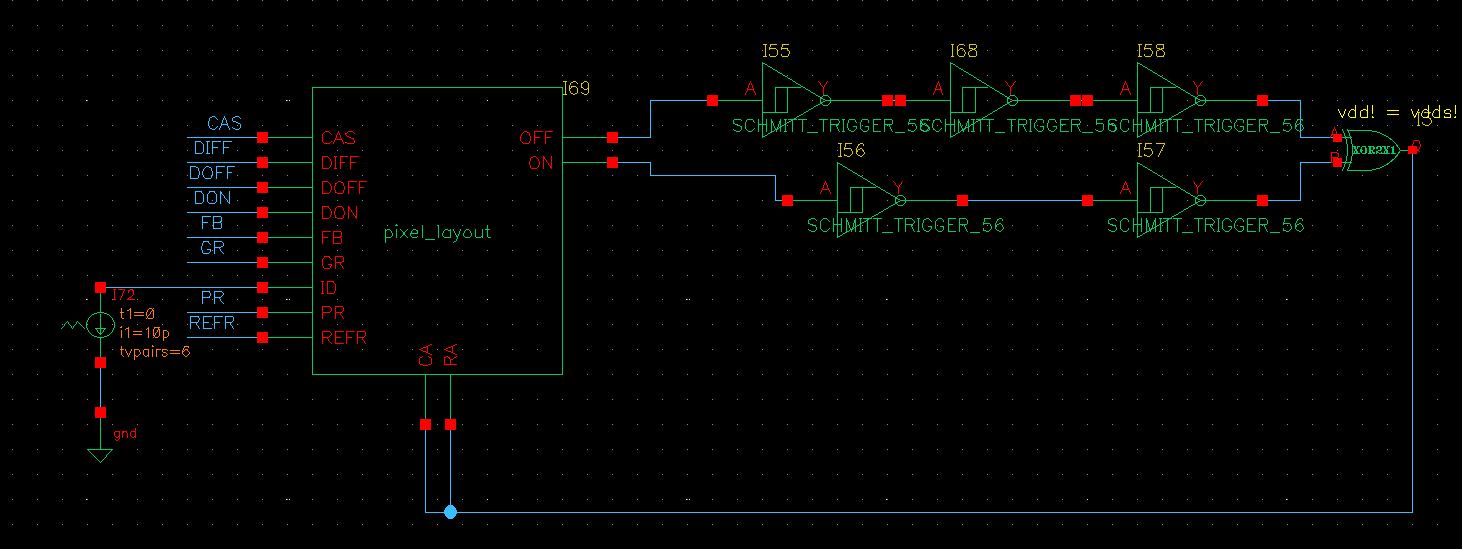
\includegraphics[width=\textwidth]{pixel_tb_pixel.png}
    \caption{Testbench for the pixel subcircuit. The ON and OFF outputs are fed back to the column and row acknowledge
    inputs to reset the circuit automatically after an event is generated. The schmidt-triggers eliminate bouncing on the
    output signals and convert the active low OFF signal to active high.}
    \label{fig:tb-pixel}
\end{figure}
\begin{figure}
    \center
    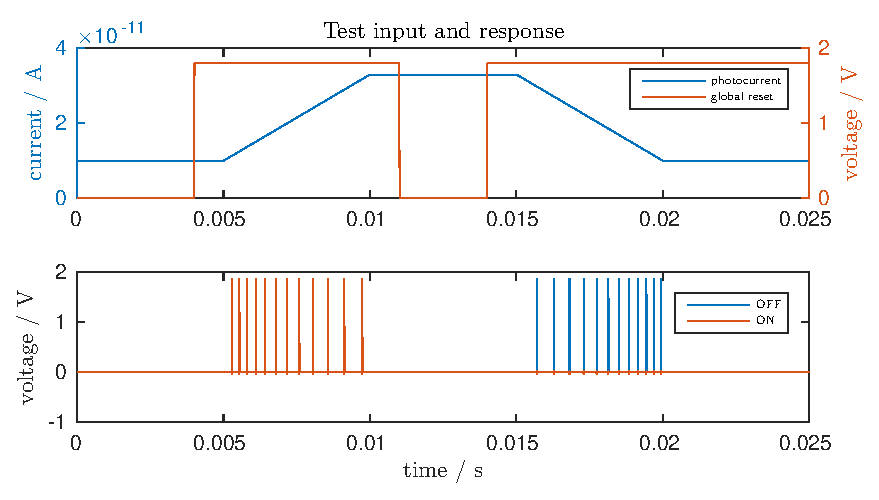
\includegraphics{pixel-response.eps}
    \caption{Testbench input and response of the pixel circuit. The pixel is reset using the global reset signal
    before both slopes so that the initial event is generated starting from the resting potential in both cases. 
    Note that the spacing between output events is logarithmic with the input current magnitude.}
    \label{fig:pixel-response}
\end{figure}
\subsection{Contrast Threshold and Mismatch Sensitivity}
We calculate the contrast threshold \(T_c\) as
\begin{equation*}
    T_c = e^{\frac{\ln(c_f)}{\mu(N_e)}} - 1
\end{equation*}
Where \(N_e\) is the (assumed normal) distribution of the  number of events generated for a factor \(c_f\) change in contrast.

We then calculate the mismatch sensitivity as the average of \(S_{on}\) and \(S_{off}\), where
\begin{equation*}
    S = \frac{e^{\frac{\ln(c_f)}{\mu(N_e)-3\sigma(N_e)}}-e^{\frac{\ln(c_f)}{\mu(N_e)+3\sigma(N_e)}}}{2}
\end{equation*}

The normally distributed number of events generated from the test input is obtained from a 200 run monte carlo 
analysis. We performed this analysis both before and after layout. The pre-layout results are shown in 
Figs.~\ref{fig:pre-on-MC} and~\ref{fig:pre-off-MC}. Here we managed to obtain zero variance in the number of generated
events. However, the post-layout results in Figs.~\ref{fig:post-on-MC} and~\ref{fig:post-off-MC} show a small variance.
This is a result of using different biases for the pre-layout schematic and the post-layout extracted schematic simulation.


The change in biases is necessary because the total gain of the differencing circuit changes as parasitic capacitance is
added to the smaller capacitor (C2=50 fF). The added parasitic capacitance is the gate capacitance of the \(M_{dp}\) transistor,
which is around 25 fF, significantly changing the capacitive divider ratio and therefore also the gain.
In order to compensate for the smaller gain, the ON and OFF biases must be set closer to the DIFF bias, but
this compromises the robustness of the circuit against mismatch. It is probably possible to get zero variation
in the number of events post-layout, but this would require adding even more capacitors, which would make the pixel
upwards of 1 mm long.

We use the biases listed in Table.~\ref{tbl:biases} and obtain a mismatch sensitivity of 0\% for the pre-layout schematic
and \(0.866\)\% for the extracted post-layout schematic.
\begin{table}
    \center
    \caption{Pre and Post-layout bias values}
    \begin{tabular}{l | c | c}
            & pre-layout & post-layout \\
        cascode & 8 nA & 8 nA \\
        diff & 60 nA & 60 nA \\
        off & 3.6 nA & 13.75 nA \\
        on & 760 nA & 356.75 nA \\
        fb & 2 nA & 2 nA \\
        pr & 1 nA & 1 nA \\
        refr & 4.4 nA & 4.4 nA \\
    \end{tabular}
    \label{tbl:biases}
\end{table}
\begin{figure}
    \center
    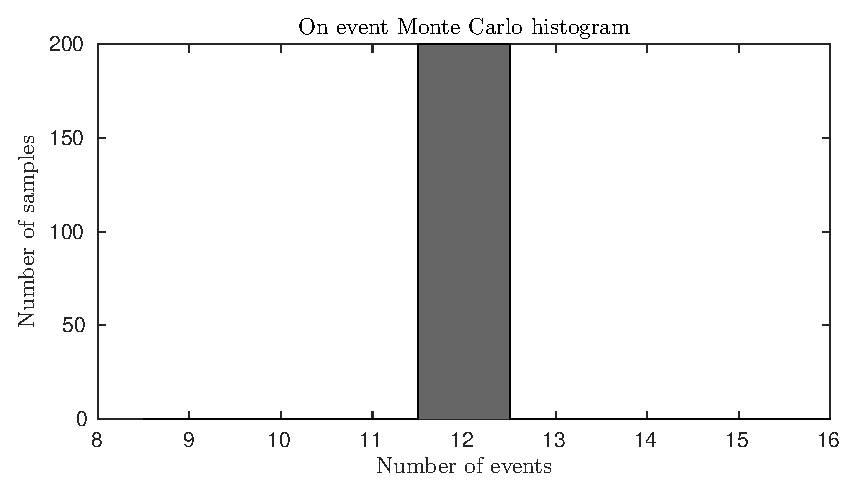
\includegraphics{pre-on-200-MC.eps}
    \caption{Histogram of the number of ON events generated by the pixel under monte carlo mismatch analysis before layout. \(\mu=12\), \(\sigma=0\).}
    \label{fig:pre-on-MC}
\end{figure}
\begin{figure}
    \center
    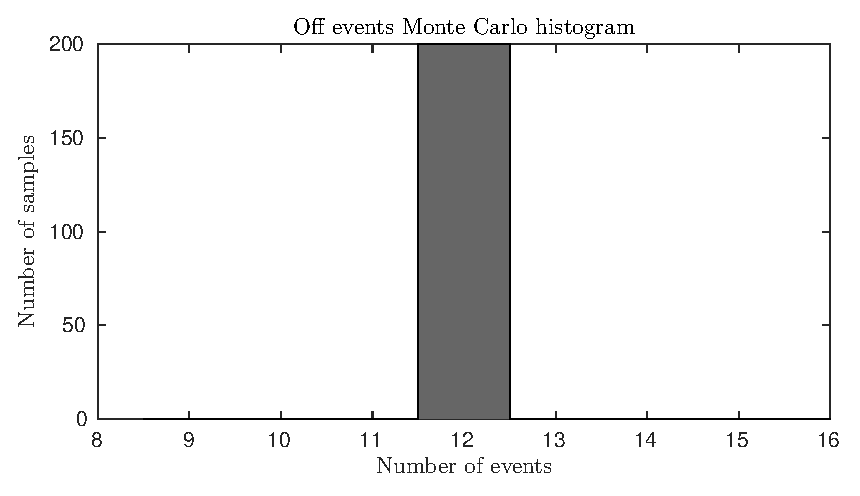
\includegraphics{pre-off-200-MC.eps}
    \caption{Histogram of the number of OFF events generated by the pixel under monte carlo mismatch analysis before layout. \(\mu=12\) \(\sigma=0\).}
    \label{fig:pre-off-MC}
\end{figure}
\begin{figure}
    \center
    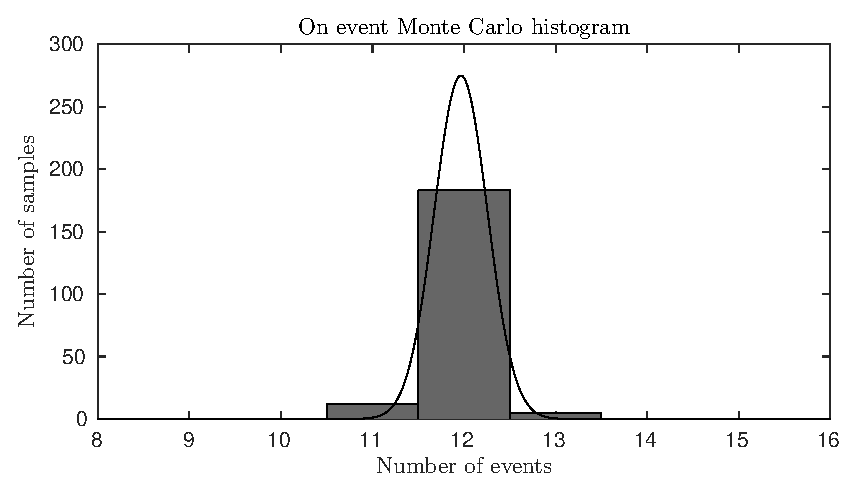
\includegraphics{post-on-200-MC.eps}
    \caption{Histogram of the number of ON events generated by the pixel under monte carlo mismatch analysis after layout. \(\mu=11.92\), \(\sigma=0.290\).}
    \label{fig:post-on-MC}
\end{figure}
\begin{figure}
    \center
    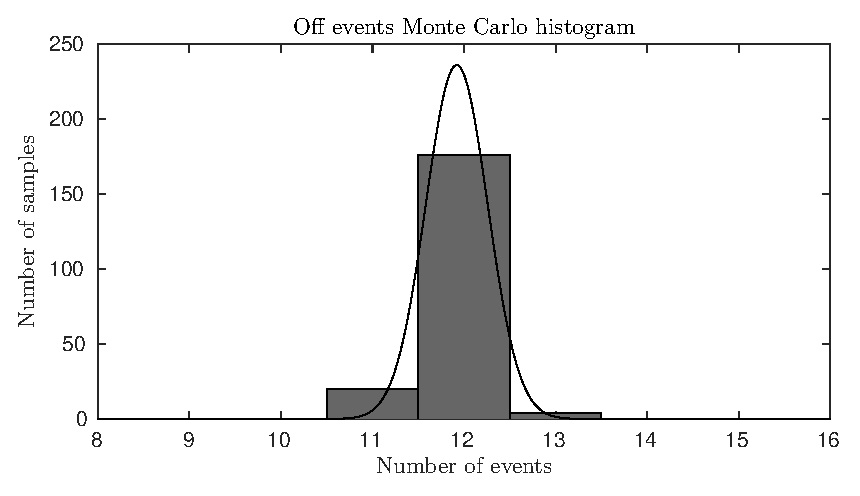
\includegraphics{post-off-200-MC.eps}
    \caption{Histogram of the number of OFF events generated by the pixel under monte carlo mismatch analysis after layout. \(\mu=11.96\), \(\sigma=0.338\).}
    \label{fig:post-off-MC}
\end{figure}
\FloatBarrier
\subsection{Power Consumption}
\subsubsection{Pre-Layout}
\begin{figure}
    \center
    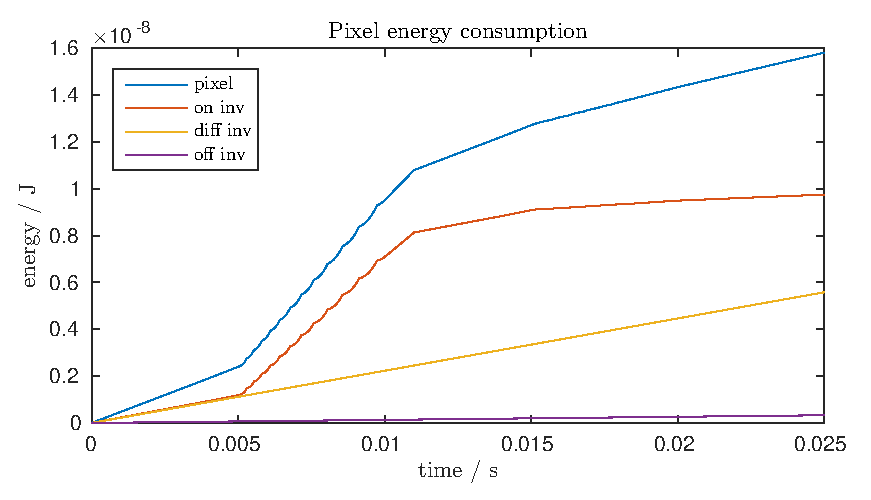
\includegraphics{pixel-power.eps}
    \caption{Cumulative energy consumed by the entire pre-layout pixel, as well as the energy consumed individually by the 
    ON, OFF and DIFF inverters. 
    The photoreceptor, source-follower and AER subcircuits consume neglible power compared to the inverters.}
    \label{fig:pixel-energy}
\end{figure}
The energy consumption of the entire pixel and the most consuming stages is shown in Fig.~\ref{fig:pixel-energy}.
From this we extract the power statistics listed in Tables.~\ref{tbl:power} and~\ref{tbl:powerpercent}.
\begin{table}[!t]
    \begin{minipage}{0.5\textwidth}
        \center
        \caption{Static and dynamic power}
        \begin{tabular}{l | c}
            & power \\
            mean & 632.4 nW \\
            static & 479.5 nW \\
            dyn. ON & 942.8 nW \\
            dyn. OFF & -154.8 nW
        \end{tabular}
        \label{tbl:power}
    \end{minipage}
    \begin{minipage}{0.5\textwidth}
        \center
        \caption{Stage power percent of total}
        \begin{tabular}{l | c}
            stage & power \% \\
            on inv & 61.69\% \\
            diff inv & 35.30 \% \\
            off inv & 2.08 \% \\
            remaining & 0.93 \%
        \end{tabular}
        \label{tbl:powerpercent}
    \end{minipage}
\end{table}
The dynamic power for off events is "negative" because the pixel consumes less power than in the static case because
the extremely power hungry ON inverter is turned off when the light intensity is dropping. The large amount of power
consumed by the ON inverter compared to the rest of the circuit is a result of the ON bias being an order of magnitude
larger than any other bias in the circuit.

We calculate the energy consumed per event as the total energy consumed when the input is in a ramping up or down,
divided by the number of events produced by the ramping input.
The energy consumed per event is 0.593 nJ for ON events and 0.135 nJ for OFF events.

\subsubsection{Post-Layout}
For the post-layout circuit, the mean power consumption is 690.6 nW, a 9\% increase. We did not obtain the power 
consumption of each stage because of difficulties in editing the extracted schematic. However, it is
reasonable to assume that the percentage of total power consumed by each stage remains about the same.

\subsection{Bandwidth}
We measured the bandwidth of the pixel circuit by replacing the reset transistors with a 15 G\(\Omega\) resistor and
the piecewise linear input current source with an AC current source. The frequency response at the \(V_{dif}\) node
is shown in Fig.~\ref{fig:freqresp}, from which we measure the bandwidth to be 23.78 kHz. 

We were unable to find the bandwidth of the post-layout extracted circuit, when calculating the FOM we will assume
that it is 10\% lower than in the ideal circuit.
\begin{figure}
    \center
    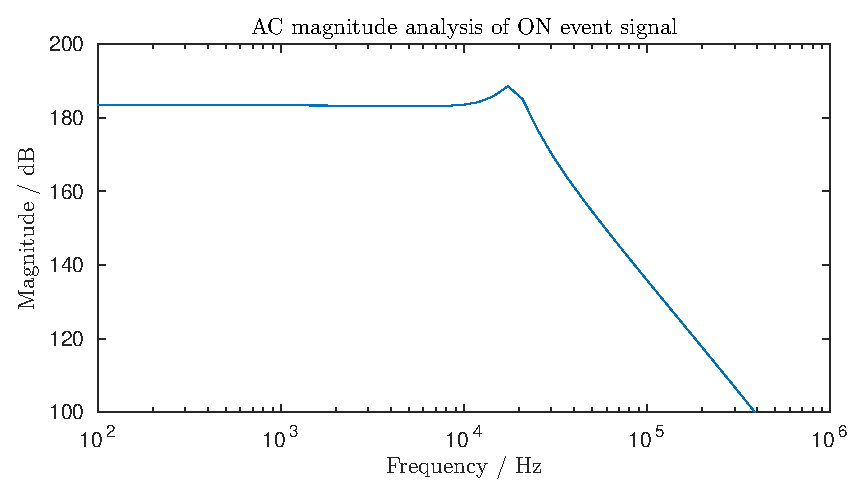
\includegraphics{pixel-bode.eps}
    \caption{Frequency response magnitude of the \(V_{dif}\) node in the pixel circuit. The -3dB bandwidth is 23.78 kHz.}
    \label{fig:freqresp}
\end{figure}

\subsection{Figure of Merit}
Evaluating eq.~\ref{eq:FOM} using our bandwidth in hertz (23780), length in feature units of 180 nm (2811.11), average power in watts (632.4 n), and 
mismatch sensitivity in percent (0), we arrive at the following pre-layout FOM
\begin{equation*}
    \text{pre-layout FOM} = \frac{23780}{632.4\cdot10^{-9}\cdot0\cdot2811.11} = \infty
\end{equation*}

And
\begin{equation*}
    \text{post-layout FOM} = \frac{21402}{690.6\cdot10^{-9}\cdot0.866\cdot2811.11} = 1.27\cdot10^7
\end{equation*}

\subsection{Fill Factor}
Our pixel has an area of 4351.6 \(\mu m^2\), of this the photodiode occupies 71.2 \(\mu m^2\), giving a fill factor of
1.64\%.
